\documentclass[tikz]{standalone}
\usepackage{cancel}
\usepackage{fontspec}
\setmonofont[]{Ubuntu Mono}

\begin{document}
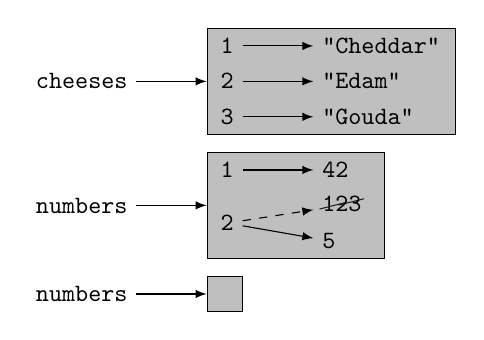
\begin{tikzpicture}[scale=0.9, transform shape]
$\node[anchor=east](ch) at(-2.75, 0) {\tt cheeses};
\node[draw, fill=lightgray, minimum width=3.5cm, minimum height=1.5cm](chv){};
\node[anchor=east] (ch1) at(-1.25, 0.5) {\tt 1};
\node[anchor=west] (chv1) at (-0.25, 0.5) {\tt "Cheddar"};
\node[anchor=east] (ch2) at(-1.25, 0) {\tt 2};
\node[anchor=west] (chv2) at (-0.25, 0) {\tt "Edam"};
\node[anchor=east] (ch3) at(-1.25, -0.5) {\tt 3};
\node[anchor=west] (chv3) at (-0.25, -0.5) {\tt "Gouda"};
\draw[-latex] (ch) -- (chv);
\draw[-latex] (ch1) -- (chv1);
\draw[-latex] (ch2) -- (chv2);
\draw[-latex] (ch3) -- (chv3);
\node[anchor=east](nu) at(-2.75, -1.75) {\tt numbers};
\node[draw, fill=lightgray, minimum width=2.5cm, minimum height=1.5cm](nuv) at(-0.5, -1.75){};
\node[anchor=east] (nu1) at(-1.25, -1.25) {\tt 1};
\node[anchor=west] (nuv1) at (-0.25, -1.25) {\tt 42};
\node[anchor=east] (nu2) at(-1.25, -2) {\tt 2};
\node[anchor=west] (nuv2) at (-0.25, -1.75) {\tt \cancel{123}};
\node[anchor=west] (nuv3) at (-0.25, -2.25) {\tt 5};
\draw[-latex] (nu) -- (nuv);
\draw[-latex] (nu1) -- (nuv1);
\draw[-latex,dashed] (nu2) -- (nuv2);
\draw[-latex] (nu2) -- (nuv3);
\node[anchor=east](em) at(-2.75, -3) {\tt numbers};
\node[draw, fill=lightgray, minimum width=0.5cm, minimum height=0.5cm](emv) at(-1.5, -3){};
\draw[-latex] (em) -- (emv);
$
\end{tikzpicture}
\end{document}
